\question[3]一质量为m的乘客乘坐竖直电梯下楼,其位移s与时间t的关系图像如图所示。乘客所受支持力的大小用$F_N$表示,速度大小用v表示。重力加速度大小为g。以下判断正确的是\key{D}\begin{center}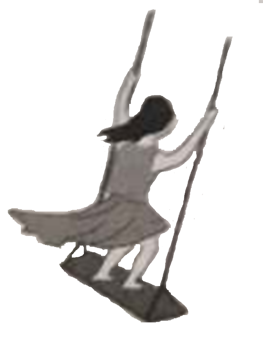
\includegraphics[width=4cm]{img/image1.png}\end{center}
\fourchoices{$0~t_1$时间内,v增大,$F_N>mg$}{$t_1~t_2$时间内,v减小,$F_N<mg$}{$t_2~t_3$时间内,v增大,$F_N<mg$}{$t_2~t_3$时间内,v减小,$F_N>mg$}
\begin{solution}{4cm}

\end{solution}



\question[3]氚核$_1^3H$发生β衰变成为氦核$_2^3He$。假设含氚材料中$_1^3H$发生β衰变产生的电子可以全部定向移动,在$3.2×10^4s$时间内形成的平均电流为$5.0×10^8A$。已知电子电荷量为$1.6×10^{-19}C$,在这段时间内发生β衰变的氚核$_1^1H$的个数为\key{B}
\fourchoices{$5.0×10^{14}$}{$1.0×10^{16}$}{$2.0×10^{16}$}{$1.0×10^{18}$}
\begin{solution}{4cm}

\end{solution}



\question[3]双缝干涉实验装置的截面图如图所示。光源S到$S_1$、$S_2$的距离相等,O点为$S_1$、$S_2$连线中垂线与光屏的交点。光源S发出的波长为λ的光,经$S_1$出射后垂直穿过玻璃片传播到O点,经$S_2$出射后直接传播到O点,由$S_1$到O点与由$S_2$到O点,光传播的时间差为Δt。玻璃片厚度为$10λ$,玻璃对该波长光的折射率为$1.5$,空气中光速为c,不计光在玻璃片内的反射。以下判断正确的是\key{A}
\fourchoices{$\Delta t=\frac{5\lambda}{c}$}{$\Delta t=\frac{15\lambda}{2c}$}{$\Delta t=\frac{10\lambda}{c}$}{$D.\Delta t=\frac{15\lambda}{c}$}
\begin{solution}{4cm}

\end{solution}


\newpage
\question[3]一列简谐横波在均匀介质中沿x轴负方向传播,已知$x=\frac{5}{4}\lambda$处质点的振动方程为$y=A\cos$($\frac{2\pi }{T}t$),则$t=\frac{3}{4}T$时刻的波形图正确的是\key{D}\begin{center}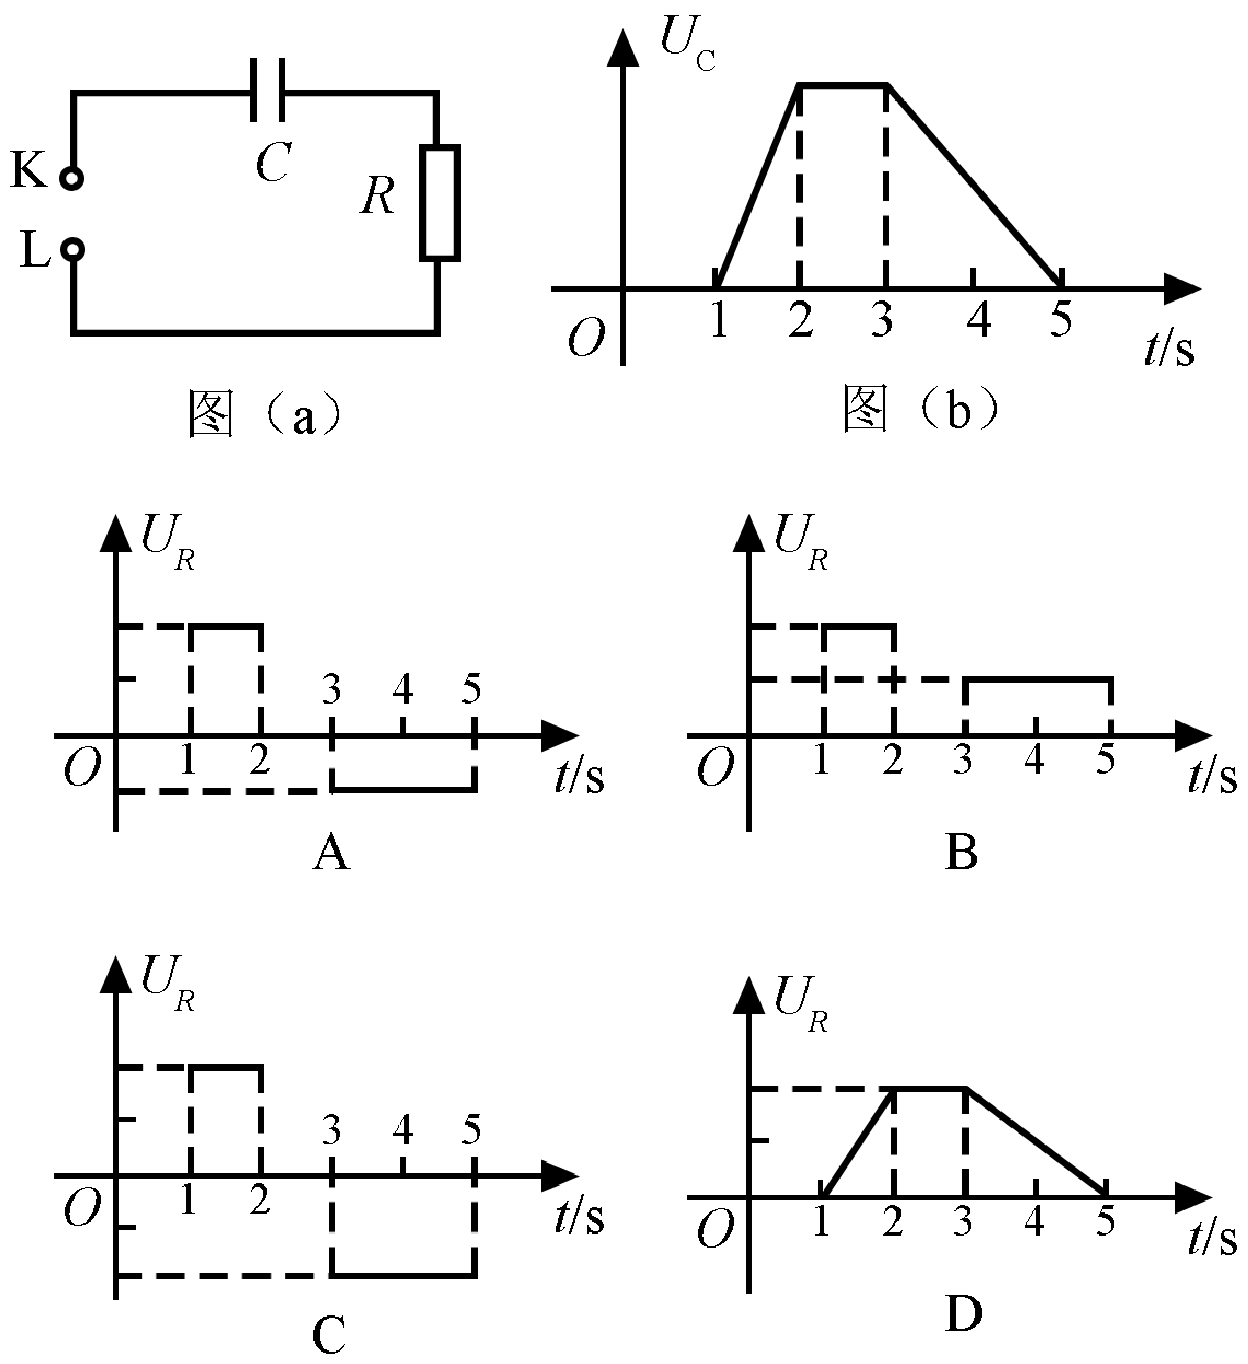
\includegraphics[width=14cm]{img/image2.png}\end{center}
\begin{solution}{4cm}

\end{solution}



\question[3]图甲中的理想变压器原、副线圈匝数比$n_1:n_2=22$:3,输入端a、b所接电压u随时间t的变化关系如图乙所示。灯泡L的电阻恒为$15Ω$,额定电压为$24V$。定值电阻$R_1=10Ω$、$R_2=5Ω$,滑动变阻器R的最大阻值为$10Ω$。为使灯泡正常工作,滑动变阻器接入电路的电阻应调节为\key{A}\begin{center}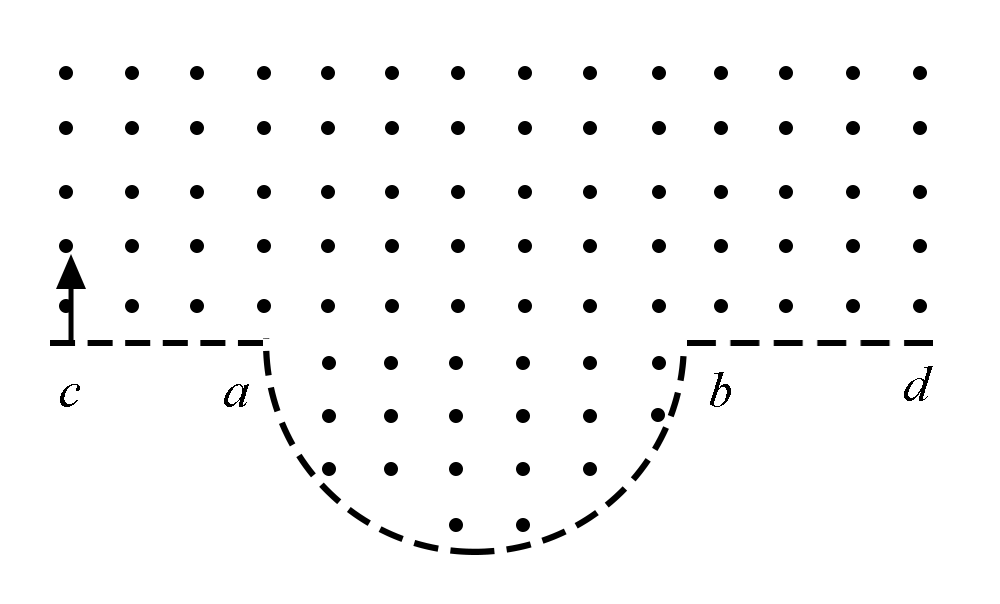
\includegraphics[width=12cm]{img/image3.png}\end{center}
\fourchoices{1Ω}{5Ω}{6Ω}{8Ω}
\begin{solution}{4cm}

\end{solution}



\question[3]一定质量的理想气体从状态a开始,经$a→b$、$b→c$、$c→a$三个过程后回到初始状态a,其$p-V$图像如图所示。已知三个状态的坐标分别为a($V_0$,$2p_0$)、b($2V_0$,$p_0$)、c($3V_0$,$2p_0$)。以下判断正确的是\key{C}\begin{center}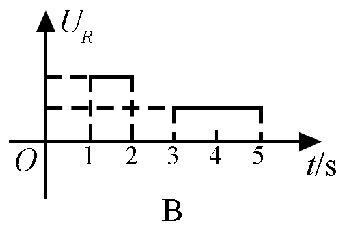
\includegraphics[width=4cm]{img/image4.png}\end{center}
\fourchoices{气体在$a→b$过程中对外界做的功小于在$b→c$过程中对外界做的功}{气体在$a→b$过程中从外界吸收的热量大于在$b→c$过程中从外界吸收的热量}{在$c→a$过程中,外界对气体做的功小于气体向外界放出的热量}{气体在$c→a$过程中内能的减少量大于$b→c$过程中内能的增加量}
\begin{solution}{4cm}

\end{solution}


\newpage
\question[3]我国将在今年择机执行"天问1号"火星探测任务。质量为m的着陆器在着陆火星前,会在火星表面附近经历一个时长为$t_0$、速度由$v_0$减速到零的过程。已知火星的质量约为地球的$0.1$倍,半径约为地球的$0.5$倍,地球表面的重力加速度大小为g,忽略火星大气阻力。若该减速过程可视为一个竖直向下的匀减速直线运动,此过程中着陆器受到的制动力大小约为\key{B}
\fourchoices{m($0.4g-\frac{v_{0}}{t_{0}}$)}{m($0.4g+\frac{v_{0}}{t_{0}}$)}{m($0.2g-\frac{v_{0}}{t_{0}}$)}{.m($0.2g+\frac{v_{0}}{t_{0}}$)}
\begin{solution}{4cm}

\end{solution}



\question[3]如图所示,一轻质光滑定滑轮固定在倾斜木板上,质量分别为m和2m的物块A、B,通过不可伸长的轻绳跨过滑轮连接,A、B间的接触面和轻绳均与木板平行。A与B间、B与木板间的动摩擦因数均为μ,设最大静摩擦力等于滑动摩擦力。当木板与水平面的夹角为$45°$时,物块A、B刚好要滑动,则μ的值为\key{C}\begin{center}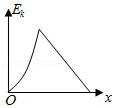
\includegraphics[width=6cm]{img/image5.png}\end{center}
\fourchoices{$\frac{1}{3}$}{$\frac{1}{4}$}{$\frac{1}{6}$}{$\frac{1}{5}$}
\begin{solution}{4cm}

\end{solution}

\end{questions}

\newpage
\group{多项选择题}{本题共 4 小题,每小题4 分。共 16 分。每小题有多个选项符合题目要求。全部选对得4分,选对但不全得2分,有选错得0分。}
\begin{questions}[30s]

\question[4]截面为等腰直角三角形的三棱镜如图甲所示。DE为嵌在三棱镜内部紧贴$BB'C^\prime C$面的线状单色可见光光源,DE与三棱镜的$ABC$面垂直,D位于线段BC的中点。图乙为图甲中$ABC$面的正视图。三棱镜对该单色光的折射率为$\sqrt{2}$,只考虑由DE直接射向侧面$AA^\prime C'C$的光线.下列说法正确的是\key{AC}\begin{center}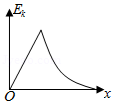
\includegraphics[width=8cm]{img/image6.png}\end{center}
\fourchoices{光从$AA^\prime C^\prime C$面出射的区域占该侧面总面积的$\frac{1}{2}$}{光从$AA^\prime C^\prime C$面出射的区域占该侧面总面积的$\frac{2}{3}$}{若DE发出的单色光频率变小,$AA^\prime C^\prime C$面有光出射的区域面积将增大}{若DE发出的单色光频率变小,$AA^\prime C^\prime C$面有光出射的区域面积将减小}
\begin{solution}{4cm}

\end{solution}



\question[4]真空中有两个固定的带正电的点电荷,电荷量不相等。一个带负电的试探电荷置于二者连线上的O点时,仅在电场力的作用下恰好保持静止状态。过O点作两正电荷连线的垂线,以O点为圆心的圆与连线和垂线分别交于a、c和b、d,如图所示.以下说法正确的是\key{BD}\begin{center}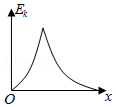
\includegraphics[]{img/image7.png}\end{center}
\fourchoices{a点电势低于O点}{b点电势低于c点}{该试探电荷在a点的电势能大于在b点的电势能}{该试探电荷在c点的电势能小于在d点的电势能}
\begin{solution}{4cm}

\end{solution}


\newpage
\question[4]如图所示,质量为M的物块A放置在光滑水平桌面上,右侧连接一固定于墙面的水平轻绳,左侧通过一倾斜轻绳跨过光滑定滑轮与一竖直轻弹簧相连。现将质量为m的钩码B挂于弹簧下端,当弹簧处于原长时,将B由静止释放,当B下降到最低点时(未着地),A对水平桌面的压力刚好为零。轻绳不可伸长,弹簧始终在弹性限度内,物块A始终处于静止状态。以下判断正确的是\key{ACD}\begin{center}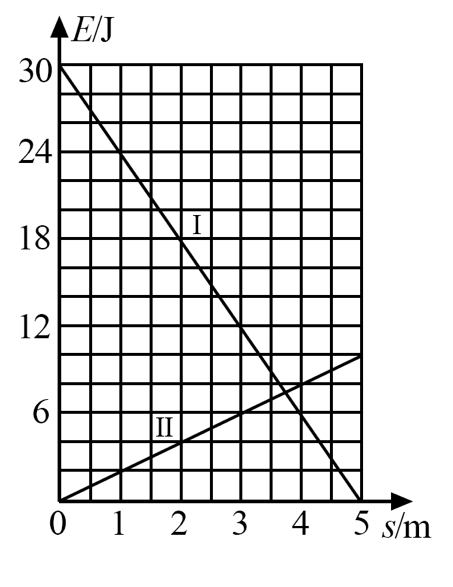
\includegraphics[]{img/image8.png}\end{center}
\fourchoices{$M<2m$}{$2m<M<3m$}{在B从释放位置运动到最低点的过程中,所受合力对B先做正功后做负功}{在B从释放位置运动到速度最大的过程中,B克服弹簧弹力做的功等于B机械能的减少量}
\begin{solution}{4cm}

\end{solution}



\question[4]如图所示,平面直角坐标系的第一和第二象限分别存在磁感应强度大小相等、方向相反且垂直于坐标平面的匀强磁场,图中虚线方格为等大正方形.一位于$Oxy$平面内的刚性导体框$abcde$在外力作用下以恒定速度沿y轴正方向运动(不发生转动).从图示位置开始计时,4s末bc边刚好进入磁场.在此过程中,导体框内感应电流的大小为I,ab边所受安培力的大小为$F_{ab}﹐$二者与时间t的关系图像可能正确的是\key{BC}
\begin{center}
    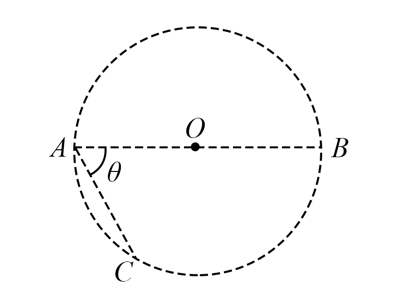
\includegraphics[]{img/image9.png}
\end{center}
\begin{center}
    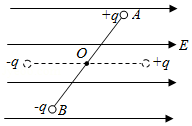
\includegraphics[]{img/image10.png}
\end{center}
\begin{solution}{4cm}

\end{solution}


\newpage
